\documentclass[11pt]{article}

\usepackage{epsilonj}
\RequirePackage{graphicx}
\RequirePackage[colorlinks,citecolor=blue,urlcolor=blue]{hyperref}

\begin{document}
	
\TITLE{Помощь любому студенту"=экономисту, или почему полезно следить за подпиской НИУ ВШЭ}
\SHORTTITLE{Помощь любому студенту"=экономисту}
\AUTHOR{}{}
\SHORTAUTHOR{}

\DoFirstPageTechnicalStuff
		
\begin{abstract}
			На дворе ноябрь, а~значит, время размышлений о~том, как подобрать релевантный материал к~курсовой. Каждый год сотни студентов НИУ ВШЭ задаются вопросом, какую тему курсовой или диплома выбрать, как грамотно подобрать материалы для написания этой работы, где найти источники публикаций. Студенты"=экономисты же сталкиваются с~проблемой подбора экономических, математических, эконометрических моделей к~теме своей работы. Будучи студенткой четвёртого курса факультета экономики, я~сталкивалась с~этой мучительной проблемой поиска и~выбора многократно, поэтому решила поделиться одним своим наблюдением со~всеми теми, кто читает этот журнал и, вероятно, будет заинтересован вопросом подбора материала к~своей работе.
		\end{abstract}
		
\begin{keyword} Econometrica, подписка, база данных, курсовая
\end{keyword}
	
	
	\section{О журнале «Econometrica»}


Признаюсь, журнал «Econometrica» стал для меня большой находкой и~палочкой"=выручалочкой при подборе материалов к~своим работам на многие темы. Мне хотелось бы более подробно рассказать о~том, чт\'{о} это за журнал и~почему я~рекомендую активно использовать его в~своей работе всем студентам, обучающимся на факультетах, связанных с~экономикой.

В~первую очередь, необходимо сказать о~том, что этот журнал публикуется в~рамках ресурса «Wiley Online Library»\footnote{\href{http://onlinelibrary.wiley.com/}{onlinelibrary.wiley.com}}\fnnsp. На эту библиотеку ВШЭ оформляет подписку каждый год, что, несомненно, не может не радовать всех тех, кто интересуется эконометрикой. Стоит также отметить, что импакт"=фактор (ИФ) журнала «Econometrica» на данный момент составляет 3{,}504. Для сравнения: ИФ таких журналов, как «\ENGs{Applied Stochastic Models in Business and Industry}» и~«\ENGs{The Econometrics Journal}» равны 0{,}532 и~1{,}128 соответственно, что, очевидно, многократно ниже значения того же показателя для рассматриваемого в~данной статье журнала.

Итак, обратимся к~самому журналу. Несомненно, одним из факторов, которые заставляют проникнуться симпатией к~данному изданию, является удобный интерфейс, о~котором позаботилась библиотека Wiley: он содержит меню поиска по журналу и~предоставляет возможность поиска по смежным темам в~других журналах, что многократно облегчает поиск нужной статьи. Его внешний вид изображён на рис.~\ref{fig:econometrica}.


\begin{figure}[htbp]
\centering  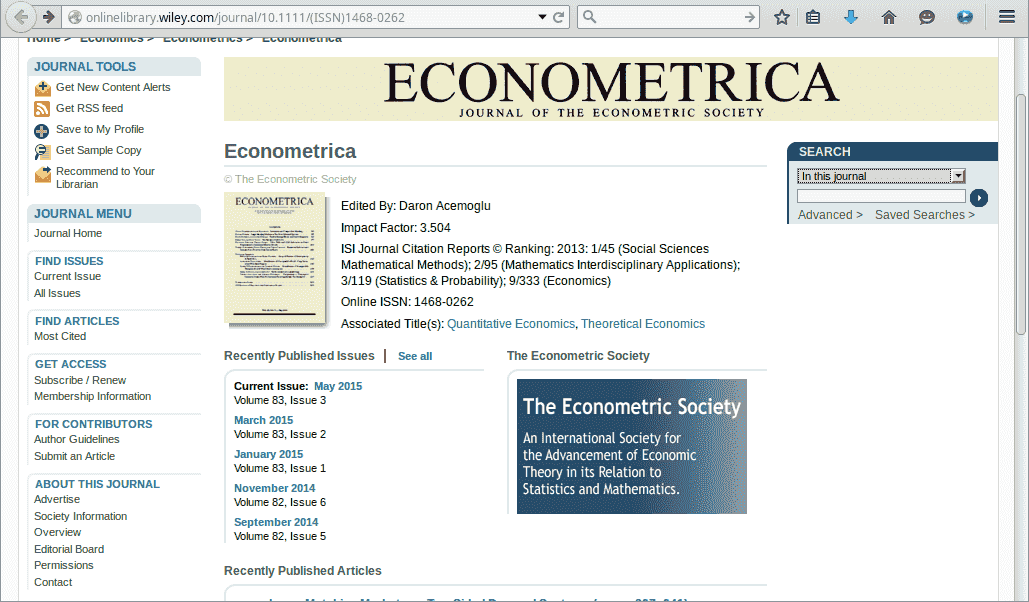
\includegraphics[width=8cm]{wiley.png}
\caption{Интерфейс журнала «Econometrica»} \label{fig:econometrica}
\end{figure}




\section{Содержание журнала}

«Econometrica» выходит раз в~два месяца и~содержит публикации членов эконометрического сообщества, которое было создано в~1930 году. Главной целью сообщество ставит публикацию исследований, связанных с~применением математического аппарата к~анализу экономических проблем и~моделей. При этом общество подчёркивает, что является независимым и~не имеет никаких требований к~полу, происхождению, политическим взглядам и~финансовому положению своих членов.

На мой взгляд, данный журнал является универсальным помощником любого студента при подготовке многих заданий, но главным образом он помогает в~деле создания курсовых и~дипломных работ. При этом важно заметить, что тематика работ связана со~многими областями и~ответвлениями экономики, поэтому почти каждый студент факультетов, связанных с~экономикой, может здесь найти интересные для себя работы.

\section{Электронный доступ}

Как найти журнал:

\begin{itemize}
	\item Зайти на сайт НИУ ВШЭ (\href{http://www.hse.ru/}{hse.ru});
	\item Перейти в~электронную библиотеку кликом по кнопке меню «Издания и~ресурсы»;
	\item В~«Бибилотеке НИУ ВШЭ» выбрать «Электронные ресурсы»;
	\item Кликнуть по «Wiley Online Library»;
	\item Ввести личные логин и~пароль;
	\item Через строку поиска найти журнал «Econometrica».
\end{itemize}


Надеюсь, мой совет облегчит жизнь многих студентов, а~кому-то, возможно, поможет определиться с~направлением исследований, которые интересны именно ему. В~любом случае, всем удачи, обилия идей для исследований и~энтузиазма!


\end{document}
